
\section{Zielsetzung}
Das Ziel des Versuchs ist es, die Funktionsweise der Wärmepumpe zu untersuchen.
Dafür werden die Güteziffer, der Massendurchsatz und die mechanische Kompressionsleistung
in Abhängigkeit von den Temperaturen und der Drücke in den Reservoirs bestimmt.
\section{Theorie}
In einem abgeschlossenen System fließt die Wärmeenergie immer vom wärmeren $T_1$
zum kälteren Medium $T_2$. Nur durch das Hinzufügen von Energie kann der Prozess
umgekehrt werden und somit Wärmeenergie auch vom kälteren zum wärmeren Körper übergehen.
Diese Energie kann zum Beispiel durch eine Wärmepumpe in das System gelangen.
\newline
Für den Wärmenergietransport zwischen zwei Medien gilt nach dem ersten Hauptsatz der Thermodynamik:
\begin{align}
  Q_1          &= Q_2 + A   \label{eqn:HS1}
\end{align}
Dieser beschreibt, dass die im wärmeren Medium aufgenommene Wärmemenge $Q_1$ gleich
der Summe der aus der im kälteren Medium entnommene Wärmemenge $Q_2$ und der zugeführten Arbeit $A$ ist.
Die Güteziffer der Wärmepumpe, welche das Verhältnis zwischen transportierter Wärmemenge
und der dazu benötigten Arbeit angibt, kann über folgende Formel berechnet werden:
\begin{equation}
  \nu = \frac{Q_1}{A}.
\end{equation}
Mit der Annahme, dass sich die Temperatur während der Wärmeübertragung nicht verändert, ergibt sich
zwischen den Wärmemengen und den Temperaturen mithilfe des 2. Hauptsatz der Thermodynamik der Zusammenhang:
\begin{equation}
  \label{eqn:HS2}
  \frac{Q_1}{T_1} - \frac{Q_2}{T_2} = 0.
\end{equation}
Dabei ist jedoch die Voraussetzung, dass der stattfindene Prozess reversibel ist.
Das bedeutet, dass die während des Zyklus aufgenommene Wärme und mechanische Energie jederzeit
vollständig zurückgewonnen werden können. Da es sich bei dieser Voraussetzung um eine idealisierte
Annahme handelt, muss für den realistischen Fall die Formel zu

\begin{equation}
  \label{eqn:2HS1}
  \frac{Q_1}{T_1} - \frac{Q_2}{T_2} > 0
\end{equation}
umformuliert werden.
Dadurch stellt sich für die reale Wärmepumpe eine andere Güteziffer $\nu_{\text{real}}$ ein.
Diese lässt sich durch die ideale Güteziffer
\begin{align}
  \nu_{id}   &= \frac{Q_1}{A} = \frac{T_1}{T_1 - T_2} \label{eqn:id}
\end{align}
zu
\begin{align}
  \nu_{real} &< \frac{Q_1}{A} = \frac{T_1}{T_1 - T_2} \label{eqn:real}
\end{align}
umschreiben.
\newline
Die Gleichung \ref{eqn:id} und \ref{eqn:real} verdeutlichen, dass die Effizienz der Wärmepumpe
größer wird, je kleiner der Temperaturunteschied zwischen den beiden Reservoirs ist.

\subsection{Bestimmung der realen Güteziffer}
Anhand der gemessenen Werte zu $T_1$ und des Zeitintervalls kann die gewonnene Wärmemenge berechnet werden:
\begin{align}
  \label{eqn:Gue}
  \frac{\increment Q_1}{\increment t} &= (m_1c_w + m_kc_k) \frac{\increment T_1}{\increment t},
\end{align}
dabei entspricht $m_1c_w$ der Wärmekapzität des Wassers in Reservoir 1 und $m_kc_k$ der Wärmekapazität
der Kupferschlange und des Eimers.
Die Güteziffer kann unter Voraussetzung der gemittelte Leistung $N$ mit
\begin{align}
    \nu  &= \frac{\increment Q_1}{\increment t N},
    \label{eqn:nu}
\end{align}
bestimmt werden.
\subsection{Bestimmung des Massendurchsatzes}
Der Massendurchsatz des Transportgases kann mit den Messwerten von $T_2$ und der Verdampfungwärme
$L$ durch
\begin{align}
  \label{eqn:masds}
  \frac{\increment Q_2}{\increment t} &= (m_2 c_W + m_k c_k) \frac{\increment T_2}{\increment t} \\
  \frac{\increment Q_2}{\increment t} &= L \frac{\increment m}{\increment t}
  \label{eqn:msds}
\end{align}
berechnet werden. Dieser gibt an wie viel Masse abhänigig von der Zeit durch das Drosselventil
gelangt.
\subsection{Bestimmung der mechanischen Kompressorleistung}
Wird ein Gas vom Volumen $V_a$ auf das Volumen $V_b$ verringert, kann die durch den Kompressor
verrichtete Arbeit durch die folgende Formel bestimmt werden:
\begin{equation}
\label{eq:mechanische_arbeit}
A_m=-\int_{V_a}^{V_b}p\mathup{d}V.
\end{equation}
Für den Kompressor wird näherungsweise davon ausgegangen, dass es sich um eine adiabatisch Kompression
handelt, bei der durch die Poissonsche Gleichung
\begin{equation}
  p_a V^{\kappa}_a = p_b V^{\kappa}_b = p V^{\kappa}
\end{equation}
der Zusammenhang zwischen Druck und Volumen beschrieben werden kann.
\newline
Im gasförmigen Zustand kann die Kompressorleisteung $N_{mech}$ mit der Dichte $\rho$ bei dem Druck $p_a$
mit
\begin{equation}
  \label{eqn:Nmech}
  N_{mech} = \frac{\increment A_m}{\increment t} =
  \frac{1}{\kappa - 1} \left( p_b \sqrt[\kappa]{\frac{p_a}{p_b}} - p_a \right)
  \frac{1}{\rho} \frac{\increment m}{\increment t}
\end{equation}
bestimmt werden.

\section{Aufbau und Durchführung}
\subsection{Aufbau}
In Abbildung \ref{fig:aufbau} ist der schematische Aufbau einer Wärmepumpe dargestellt.
\begin{figure}
\centering
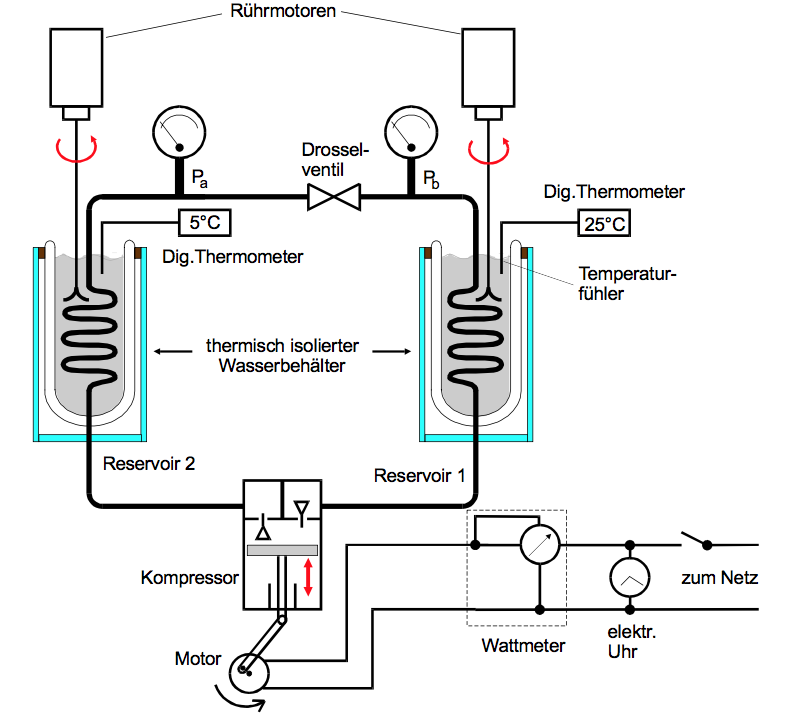
\includegraphics[width=0.7\textwidth]{aufbau.png}
\caption{Schematischer Aufbau einer Wärmepumpe}\cite{on1}
\label{fig:aufbau}
\end{figure}
\newline
Als Wärmetransportmittel wird in der Wärmepumpe das reale Gas Dichlodifluormethan genutzt.
Der Kompresser erzeugt einen Kreislauf des Systems, indem der Aggregatszustand des Gases
von gasförmig zu flüssig und umgekehrt von ihm beeinflusst wird.
\newline
Durch das Drosselventil wird ein Druckunterschied zwischen $p_a$ und $p_b$ erzeugt.
Unter der Temperatur $T_1$ und dem Druck $p_b$ ist das Gas flüssig und unter der Temperatur $T_2$
und dem Druck $p_a$ gasförmig. Außerdem dient das Drosselventil der Wärmepumpe als Steuerungsvorrichtung.
Es sorgt dafür, dass kein flüssiges Gas in den Kompressor gelangt, sondern nur gasförmiges.
Um eine eine blasenfreie Flüssigkeitszufuhr in das Drosselventil zu gewährleisten, fließt
das verflüssigte Gas zuerst durch einen Reiniger.
\newline
Im wärmeabgebenden Reservoir $2$ verdampft das Gas bei der Aufnahme der Verdampfungswärme $L$.
Danach wird es im Kompressor adiabatisch komprimiert, was zu einem Wiederanstieg von Druck und Temperatur des Gases führt.
In wärmeaufnehmende Reservoir $1$ erhöht sich die Temperatur, da das Gas während des Verflüssigens eine Kondensationswärme
abgibt. Dies führt zu einer Temperaturabnahme in Reservoir $2$.

\subsection{Durchführung}
Vor dem Beginn des Versuchs werden die beiden Reservoirs mithilfe eines Messkolbens mit je $3$\, Liter
Wasser befüllt. Nach Einschalten des Kompressors werden im Minutentakt von den Reservoirs 1 und 2 die
Temperaturen $T_1$ und $T_2$, die Drücke $p_a$ und $p_b$ und die Leistungsaufnahme des Kompressors $A$
gemessen und notiert. Dies geschieht solange, bis $T_1$ einen Wert von $50\si{\degreeCelsius}$ erreicht.
